\documentclass[10pt]{beamer}

\usetheme[progressbar=frametitle]{metropolis}
\usepackage{appendixnumberbeamer}

\usepackage{animate}
\usepackage{verbatim}
\usepackage{graphicx}

\usepackage{booktabs}
\usepackage[scale=2]{ccicons}

\usepackage{pgfplots}
\usepgfplotslibrary{dateplot}

\usepackage{xspace}
\newcommand{\themename}{\textbf{\textsc{metropolis}}\xspace}

\title{Network Cloning using DNA Barcodes}
\subtitle{Locally copying connectivity information}
% \date{\today}
\author{Batuhan Baserdem \\ Alexei Koulakov \\ Sergey Shuvaev \\ Tony Zador}
\institute{Cold Spring Harbor Laboratory}
\titlegraphic{\hfill\includegraphics[width=0.5\textwidth]{png/cshl_long.png}}

\begin{document}

\maketitle

\begin{frame}{Outline}
  \setbeamertemplate{section in toc}[sections numbered]
  \tableofcontents
\end{frame}

%-----MOTIVATION CHAPTER-----%
\section{Motivation}

\begin{frame}[fragile]{DNA Barcodes}
    % Explain what are DNA barcodes here
    How to get connectivity information of the brain \\
    Using colors (\textasciitilde 3 colors) vs tags (potentially $\inf$)\\
    Using SYNseq \cite{synseq} allows for tagging neurons.
    \begin{center}
        \includegraphics[width=0.9\textwidth]{png/synseq.png}
    \end{center}
\end{frame}

\begin{frame}[fragile]{Connectivity Reconstruction}
    Can be reconstruct as a matrix. \\
    Can it be reconstructed inside another network directly?
    \begin{center}
        \includegraphics[width=0.9\textwidth]{png/reconst_flow.png} \\
        Tabula Rasa (TR) network: All-to-all connected network
    \end{center}
    \onslide<2>{Viable method to encode connectivity data in DNA}
\end{frame}

\begin{frame}{Viable Algorithm}
    \begin{center}
        \includegraphics[width=0.9\textwidth]{png/state_explain.png}
    \end{center}
    \begin{enumerate}
        \item Express barcodes in original network
        \item Express sequences of barcode pairs
        \item<2-> Put barcode-pairs on a TR network such that it sits on synapses.
        \item<3-> Shave off unoccupied synapses.
    \end{enumerate}
\end{frame}

\begin{frame}[fragile]{Nonlocality}
    % Why would it be interesting?
    \begin{center}
        \includegraphics[width=0.9\textwidth]{png/conn_nonlocal.png}
    \end{center}
    \metroset{block=fill}
    \begin{alertblock}{Requires Supervisor}<2->
        Inherently non-local algorithm.
        Supervisor needs knowledge of all neurons simultaneously.
    \end{alertblock}
    \begin{alertblock}{Artificial Neural Nets (ANN)}<3->
        Can have their matrices copied, but this action is also non-local.
    \end{alertblock}
\end{frame}

\begin{frame}[fragile]{Local Algorithm}
    \begin{itemize}
        \item Should make use of only local information. (Each cell should only know it's synapses)
        \item Cannot use a supervisor.
    \end{itemize}
    \metroset{block=fill}
    \begin{exampleblock}{\centering Is local algorithm possible?}<2->
        \centering
        And is it guaranteed to converge?
    \end{exampleblock}
\end{frame}

%-----MOTIVATION CHAPTER-----%



%-----THEORY CHAPTER-----%
\section{Theory}

\begin{frame}[fragile]{Algorithm}
    \begin{enumerate}
        \item Try to move barcode-pairs randomly.
        \item Have some local rule to accept or refuse moves.
        \item<2-> Reach one-barcode-one-cell (OBOC)
        \item<3-> Prune empty synapses
    \end{enumerate}
    \metroset{block=fill}
    \begin{exampleblock}{Locality Constraint:}<4->
        As long as acceptance uses local information, (cells that are adjacent
        to the synapse of interest) algorthm will be local.
    \end{exampleblock}
    \begin{block}{OBOC State:}<5->
        If an OBOC state is reached, then there is a one-to-one mapping between
        cells of the original connectome and the cells of the new connectome.
    \end{block}
\end{frame}

\begin{frame}[fragile]{Simulated Annealing (SA)}
    \begin{itemize}
        \item Propose a state change (chosen randomly).
        \item Calculate change of system energy
        \item If energy decreases, accept state change.
        \item If energy increases, have a chance to accept new state with some temperature. ($p=e^{-\delta E / T}$)
        \item Gradually reduce temperature to 0.
    \end{itemize}
    \begin{alertblock}{\centering High Temperature}<2->
        Allows searching for global features in the state-space,
        and kicks system out of \textit{shallow} local minima.
    \end{alertblock}
    \begin{exampleblock}{\centering Low Temperature}<3->
        Once temperature is low, motion in state space is constraint further
        towards a minima. \\
        Once T=0, only moves which decrease energy are allowed.
    \end{exampleblock}
    \metroset{block=fill}
    \begin{block}{Locality}<4->
        If Hamiltonian is local, then the SA method is a local method.
    \end{block}
\end{frame}

\begin{frame}{Local Hamiltonian}
    \begin{equation*}
        \centering
        H = \sum^{N}_{n=1} \left[
        - \left( 1 + \epsilon \right) \sum^{B}_{\beta=1}
        \left( C_{n , \beta} \right)^\gamma +
        \epsilon \left( \sum^{B}_{\beta=1} C_{n , \beta} \right)^\gamma
        \right]
    \end{equation*}
    \begin{columns}[T,onlytextwidth]
        \column{0.5\textwidth}
        \metroset{block=fill}
        \begin{exampleblock}{\centering $C_{n, \beta}$}<2->
            \begin{itemize}
                \item State variable.
                \item Number of barcodes $\beta$ in cell $n$.
            \end{itemize}
        \end{exampleblock}
        \begin{exampleblock}{\centering $\mathbb{\gamma}$ (=2)}<3->
            \begin{itemize}
                \item Parameter
                \item Must be $>1$
                \item Value 2 used for proofs.
            \end{itemize}
        \end{exampleblock}

        \column{0.1\textwidth}

        \column{0.4\textwidth}
        \metroset{block=fill}
        \begin{exampleblock}{\centering $\mathbb{\epsilon}$ (=10)}<4->
            \begin{itemize}
                \item Parameter
                \item Cost associated with multiple labels
                \item Enforces OBOC state
            \end{itemize}
        \end{exampleblock}
        \begin{itemize}
            \item<5-> N = Number of cells in TR network
            \item<5-> B = Number of unique barcodes
        \end{itemize}
    \end{columns}
\end{frame}

\begin{frame}{Hamiltonian - 1\textsuperscript{st} Term}
    \begin{equation*}
        \centering
        H^1 =
        - \left( 1 + \epsilon \right)
        \sum^{N}_{n=1} \sum^{B}_{\beta=1}
        \left( C_{n,\beta} \right) ^ 2
    \end{equation*}
    \begin{alertblock}{\centering Sparsity term}<2->
        \centering
        Forces sparse representation. \\
        As long as it is a superlinear ($\gamma>1$) function,
        barcodes of the same type will be \textit{attracted} together.
    \end{alertblock}
\end{frame}

\begin{frame}{Hamiltonian - 2\textsuperscript{nd} Term}
    \begin{equation*}
        \centering
        H^2 =
        \epsilon \times
        \sum^{N}_{n=1} \left( \sum^{B}_{\beta=1}
        C_{n,\beta} \right) ^ 2
    \end{equation*}
    \begin{alertblock}{\centering Cost term}<2->
        Since multiplier $\epsilon<1+\epsilon$, doesn't overpower 1\textsuperscript{st} term. \\
        Causes \textit{repulsion} between barcode clumps.
    \end{alertblock}
    \metroset{block=fill}
    \only<3>{
        \begin{exampleblock}{\centering When $\epsilon = 0$ ($H^2 = 0$)}
            \begin{columns}[T,onlytextwidth]
                \column{0.5\textwidth}
                \includegraphics[width=\textwidth]{png/correct_config.png} \\
                $H^1 = - 2^2_{n=1} + -2^2_{n=2} = -8$
                \column{0.5\textwidth}
                \includegraphics[width=\textwidth]{png/false_config.png} \\
                $H^1 = - (2^2_{\beta=A} + -2^2_{\beta=D})_{n=1} = -8$
            \end{columns}
            \centering
            Without $\epsilon$, states have the same energy.
        \end{exampleblock}
    }
    \begin{exampleblock}{\centering When $\epsilon > 0$}<4-5>
        \begin{columns}[T,onlytextwidth]
            \column{0.5\textwidth}
            \includegraphics[width=\textwidth]{png/correct_config.png} \\
            \only<4>{
                $H^1 = -(1+\epsilon)8$ \\
                $H^2 = \epsilon ( 2^2_{n=1} + 2^2_{n=2}) = 8 \epsilon$
            }
            \only<5>{ $H = -8(1+\epsilon) + 8\epsilon = -8$ }
            \column{0.5\textwidth}
            \includegraphics[width=\textwidth]{png/false_config.png} \\
            \only<4>{
                $H^1 = -(1+\epsilon)8$ \\
                $H^2 = \epsilon 4_{n=1}^2 = 16 \epsilon$
            }
            \only<5>{ $H = -8(1+\epsilon) + 16\epsilon = -8 + 8\epsilon$ }
        \end{columns}
        \only<5>{
            \centering
            Hamiltonians are distinct, OBOC state is lower energy.
        }
    \end{exampleblock}
\end{frame}

\begin{frame}{Moves: State Changes}
    We consider three different \textit{moves}, the way the barcode-pair to
    synapse correspondance can change at a given time. \\
    ($\rho$ stands for connection density: \# of barcode-pairs / \# possible
    barcode-pair combinations.) \\
    \begin{columns}[T,onlytextwidth]
        \metroset{block=fill}
        \column{0.33\textwidth}
        \begin{exampleblock}{Jump}<2->
            A barcode-pair detaches from a synapse, and moves to another one
            through a cell.
        \end{exampleblock}
        \column{0.33\textwidth}
        \begin{exampleblock}{Flip}<3->
            A barcode-pair passes to the synapse of opposite polarity. \\
            Can be viewed as a compound of two jumps with a probability $\rho-1/N$.
        \end{exampleblock}
        \column{0.33\textwidth}
        \begin{exampleblock}{Swap}<4->
            Two barcode-pairs (that share a cell) swap their positions.
            Can be viewed as a compound of two jumps with a probability $1/N$.
        \end{exampleblock}
    \end{columns}
    \only<5> {
        \centering
        Probabilities
        \begin{columns}[T,onlytextwidth]
            \column{0.33\textwidth}
            \centering
            $1-\rho$
            \column{0.33\textwidth}
            \centering
            $\rho-1/N$
            \column{0.33\textwidth}
            \centering
            $1/N$
        \end{columns}
    }
\end{frame}

\begin{frame}[fragile]{Moves}
    \begin{center}
        \includegraphics[width=0.9\textwidth]{png/conn_local.png}
    \end{center}
\end{frame}

\begin{frame}[fragile]{Convergence}
    \metroset{block=fill}
    \begin{exampleblock}{Converges to OBOC}
        It is proven ($\gamma=2$, $\epsilon>0$) for a non-OBOC state, there is
        at least one move that strictly lowers the energy of the system. \\
        Thus ground state (GS) has to be an OBOC state.
    \end{exampleblock}
    \begin{exampleblock}{OBOC is isomorphic to original connectome}
        It is proven that if OBOC state is reached, the mapping between cells of
        old connectome and the new connectome preserve connectivity
    \end{exampleblock}
    \begin{alertblock}{\centering Ground State Degeneracy}<2->
        All OBOC states are permutations of each other. \\
        Thus all OBOC states are equally good solutions.
        \begin{center}
            \includegraphics[width=0.5\textwidth]{png/global_local.png}
        \end{center}
    \end{alertblock}
\end{frame}
%-----THEORY CHAPTER-----%



%-----RESULTS CHAPTER-----%
\section{Results}

\begin{frame}[fragile]{Simulation}
    We used MATLAB to simulate runs of the algorithm
    \begin{enumerate}
        \item Generate a random network of desired $N$,$\rho$. \textit{Erdős–Rényi (ER)}
        \item Extract barcode-pair (netlist) representation.
        \item Place barcode-pairs randomly on TR network.
        \item Run SA until energy reaches GS
        \item Prune TR network, and check graph isomorphism.
    \end{enumerate}
    \metroset{block=fill}
    \begin{alertblock}{\centering Limitation}
        Non-parallelisable; (every SA step depends on previous)
        thus runtime gets really long.
    \end{alertblock}
\end{frame}

\begin{frame}[fragile]{Parameters}
    \begin{itemize}
        \item[$T$] Lowered linearly $10^{-2}$ to $10^{-6}$. (Using
            projected runtime from previous runs)
        \item[$\epsilon$] Fixed at 10
        \item[$\gamma$] Fixed at 2
        \item[$N$] Varied (logarithmically) from $10$ to $1000$
        \item[$\rho$] VAried (logarithmically) from $0.05$ to $0.8$
    \end{itemize}
\end{frame}

% Disable animation for faster compilation
\begin{comment}
\begin{frame}[fragile]{Animation: N = 10}
    \begin{columns}[T,onlytextwidth]
        \column{0.5\textwidth}
        \animategraphics[loop,controls,width=\textwidth]{15}{video/fortex/run10-}{0}{89}
        \column{0.4\textwidth}
        \begin{itemize}
            \item Orange: False connection
            \item Blue: Missing connection
            \item Green: Correct connection
        \end{itemize}
    \end{columns}
\end{frame}

\begin{frame}[fragile]{Animation: N=50}
    \begin{center}
        \animategraphics[loop,controls,width=0.5\textwidth]{15}{video/fortex/run50-}{0}{94}
    \end{center}
\end{frame}

\begin{frame}[fragile]{Animation: N=500}
    \begin{center}
        \animategraphics[loop,controls,width=0.5\textwidth]{15}{video/fortex/run500-}{0}{101}
    \end{center}
\end{frame}

\begin{frame}[fragile]{Real-Time Animation, N=10}
    \begin{center}
        \animategraphics[loop,controls,width=\textwidth]{2}{video/fortex/realtime10-}{0}{21}
    \end{center}
\end{frame}
\end{comment}

\begin{frame}{Convergence Plot}
    \centering
    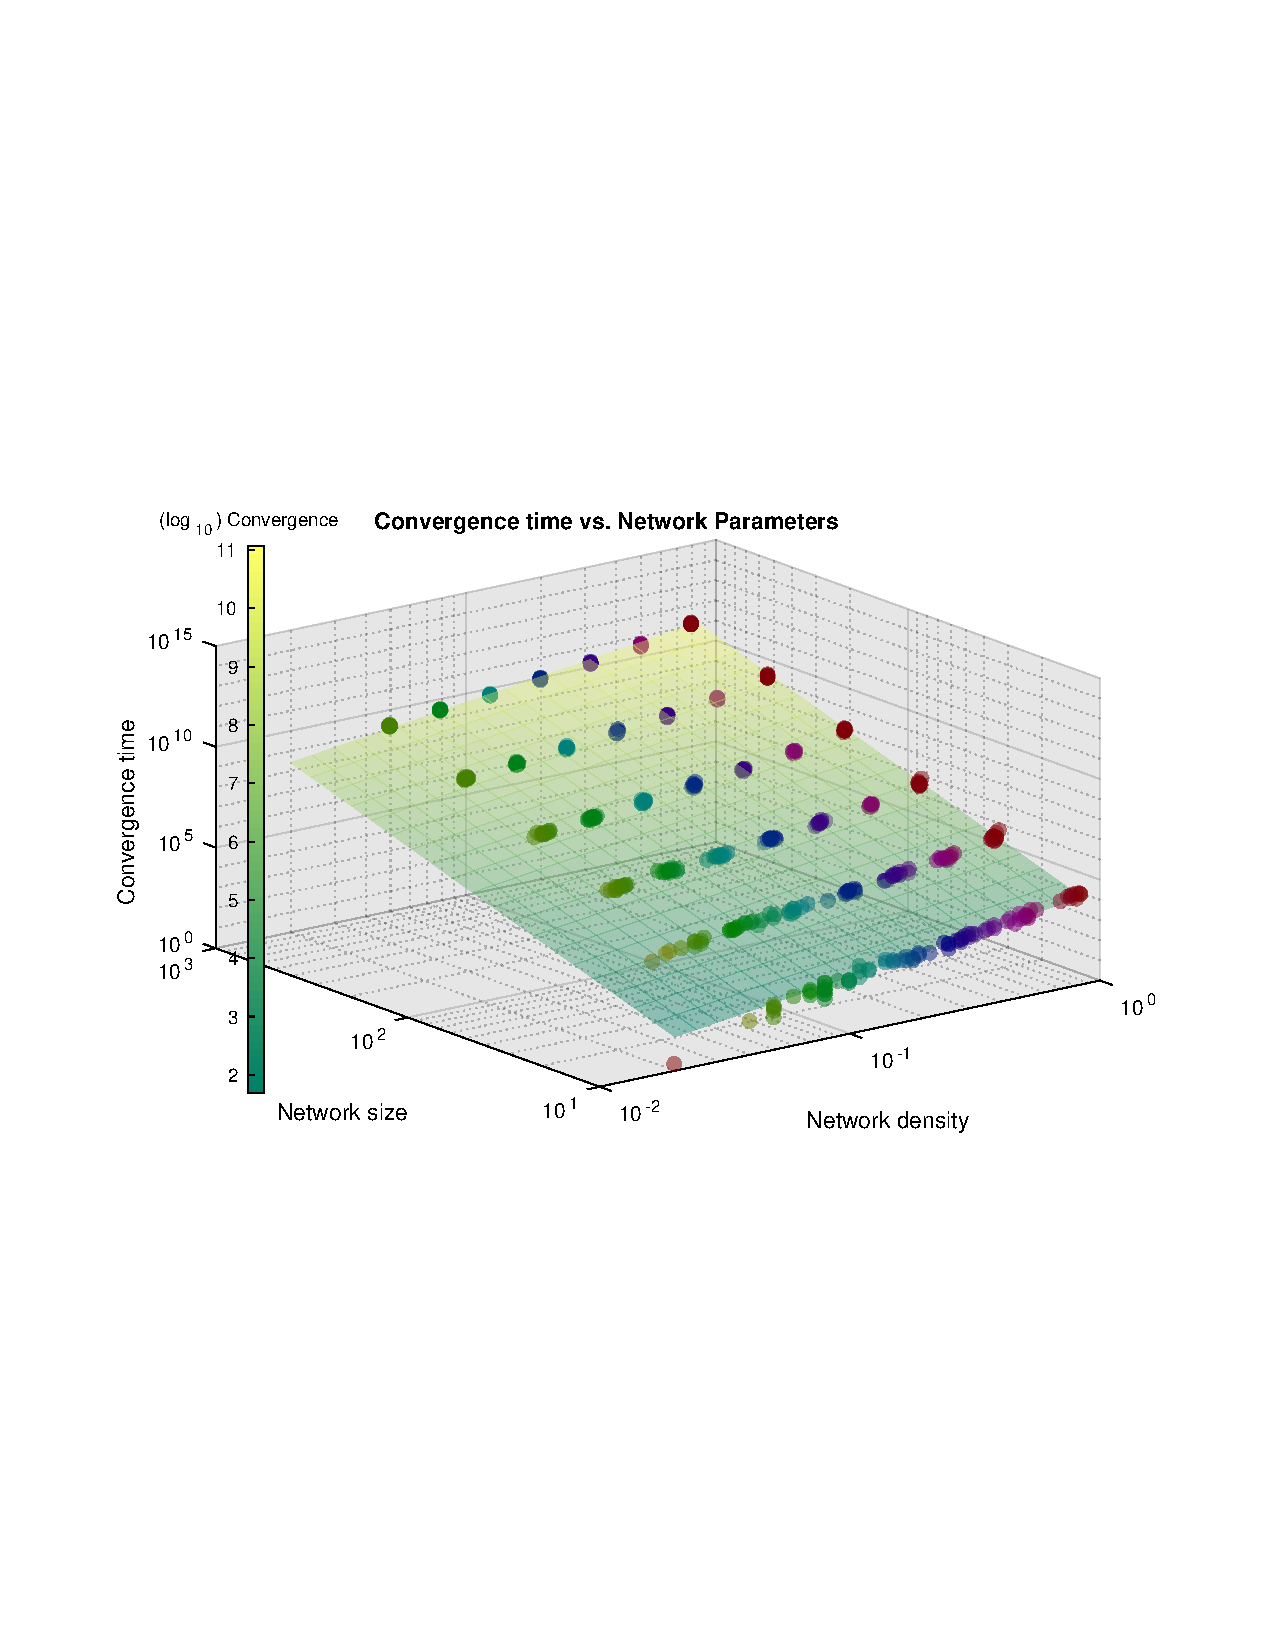
\includegraphics[width=\textwidth]{png/convergence_3d_10-1000.png}
\end{frame}

\begin{frame}{Regression}
    \begin{equation*}
        \centering
        C = 12.43 \times \rho^{1.63} \times N^{3.37}
    \end{equation*}
    Number of steps for convergence is described well by a power law dependence
    on N. \\ Due to the small range of $\rho$ $(0,1)$, most functions will fit.
\end{frame}

\begin{frame}{Convergence Plot: 2D}
    \includegraphics[width=\textwidth]{png/data_conv_sizecol.png}
\end{frame}

\begin{frame}{Convergence Plot: 2D}
    \includegraphics[width=\textwidth]{png/data_conv_denscol.png}
\end{frame}
%-----RESULTS CHAPTER-----%

%-----COCNLUSION CHAPTER-----%
\section{Conclusion}

\begin{frame}[fragile]{Remarks}
    \begin{itemize}
        \item SA is a viable tool to generate connectome locally from a netlist
            representation. Convergence is guaranteed.
        \item Convergence time of such an algorithm is polynomial on network
            size and density.
        \item Low level connectivity information can be encoded and recovered
            from DNA sequences in a biologically plausable way.
    \end{itemize}
\end{frame}

\begin{frame}
    Thank you for listening!
\end{frame}

\begin{frame}[allowframebreaks]{References}
  \bibliography{presentation}
  \bibliographystyle{ieeetr}
\end{frame}
%-----CONCLUSION CHAPTER-----%

\appendix

\end{document}

